\chapter{Retrospective Loss: Looking Back to Improve Training of Deep Neural Networks}

Adobe \\

\textbf{Reference:}~\cite{jandial2020retrospective}

\textbf{Keywords:} neural networks, loss functions

\section*{Какую задачу решают авторы?}

В статье демонстрируется простой способ улучшить качество практически любой нейросетевой архитектуры. \\

Улучшение достигается путем добавления к функции потерь дополнительного слагаемого (retrospective loss).

При оптимизации Retrospective loss вместе с основной функцией потерь, учитываются предыдущие состояния параметров модели таким образом, чтобы как можно быстрее двигаться в направлении к оптимальным параметрам. \\

В статье изложена мотивация стоящая за retrospective loss, теоретическое обоснование того почему ее использование дает преимущества, и большое количество экспериментов на разных задачах, демонстрирующих улучшение качества моделей. 

\section*{Как решают?}

Рассмотрим сначала как выглядит retrospective loss

\ddef{Retrospective Loss}{
\label{def:retrospective_loss}
Given network  $g \colon \bR^n \to \bR^d$ parametrized by its weights $\theta$ an input data-label pair $(\vecx_i,y_i)$, the retrospective loss at time step $T$ is given by:
\begin{equation*}
    \mathcal{L}_{retrospective} = (\kappa+1) \| g_{\theta^T}(\vecx_i) - y_i \| - \kappa \| g_{\theta^T}(\vecx_i) - g_{\theta^{T_p}}(\vecx_i) \| 
\end{equation*}
where $\kappa$ - scaling co-efficients, $\theta^T$ - parameters at time step $T$ and $T_p$ - previous time step.
}

\paragraph{Интуиция} Минимизируя $\mathcal{L}_{retrospective}$ мы пытаемся сделать так, чтобы на очередном шаге предсказание модели для $\vecx_i$ было ближе к $y_i$, чем к предыдущему предсказанию. \\

Рисунок~\ref{fig:geom_intuition} визулизирует данную интуицию. 

По определению, $\mathcal{L}_{retrospective} < 0$ в ситуации, когда предсказание в текущем состоянии, $g_{\theta^T}$, ближе к $y_i \coloneqq g_{\theta^{*}}$, чем к предыдущему предсказанию $g_{\theta^{T_p}}$. 

В результате, пространство параметров делиться на две части - первая где $\mathcal{L}_{retrospective} < 0$, и  вторая где $\mathcal{L}_{retrospective} \geq 0$. \\

Minimizing retrospective loss pushes the network towards parameters further inside the polytope, thus helping speed up the training process. \\

\begin{figure}
    \centering
    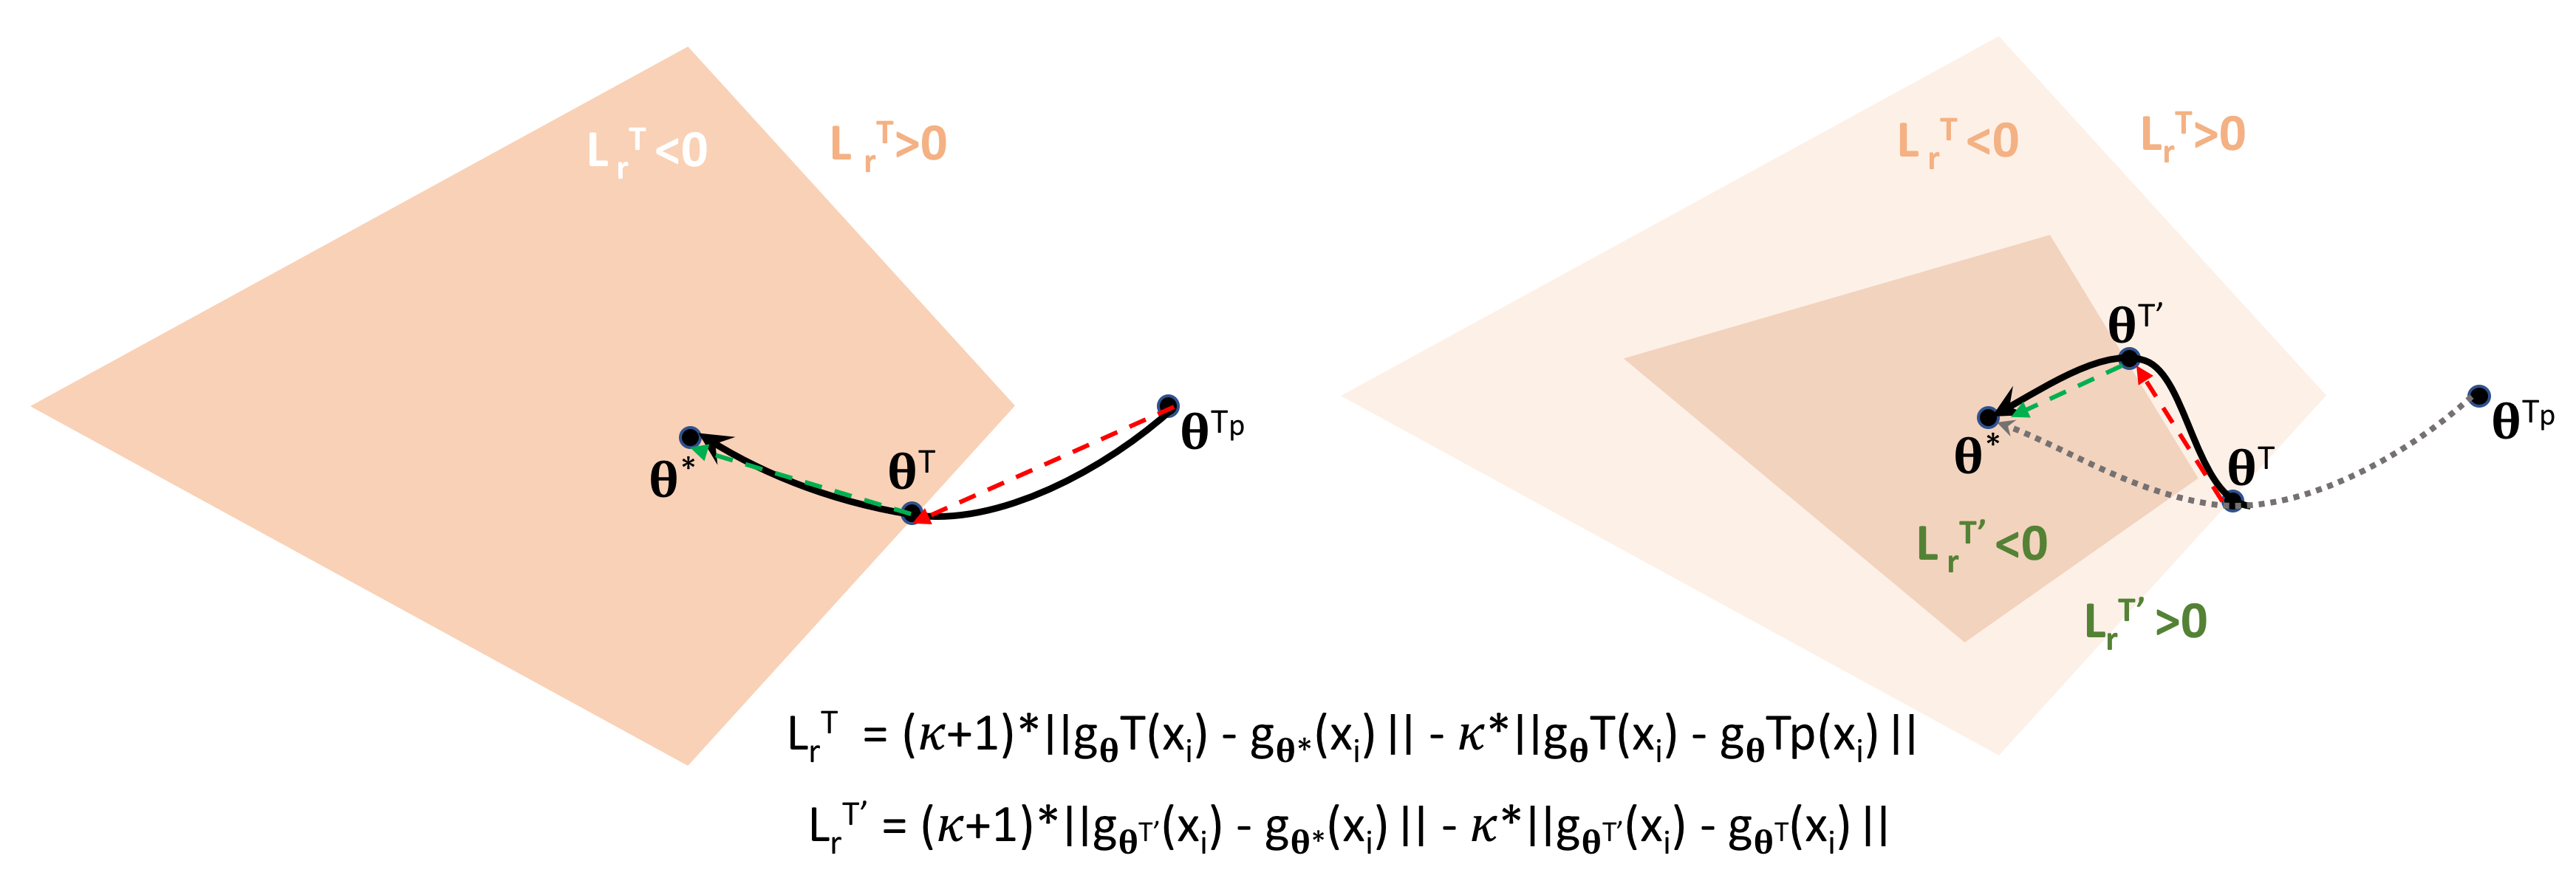
\includegraphics[width=0.8\linewidth]{images/dualing_loss_viz.png}
    \caption{Geometric intuition of the working of the proposed retrospective loss.}
    \label{fig:geom_intuition}
\end{figure}

Новый loss - просто сумма $\mathcal{L}_{task}$ и $\mathcal{L}_{retrospective}$. 

\paragraph{Анализ} Главный вопрос: почему добавление $\mathcal{L}_{retrospective}$ позволяет ускорить обучение? \\

Для ответа на этот вопрос авторы вводят следующее определение

\ddef{Consistency of Loss Terms for Neural Network Models}{
Пусть $g_{\theta}$ нейросеть с параметрами $\theta$ и $\theta^{*} \coloneqq \argmin_{\theta} \mathcal{L}_{task} $ - решение задачи.

Тогда если при добавлении к $\mathcal{L}_{task}$ функции $\mathcal{L}_{add}$, с целью ускорить обучение, оптимум достигается в той же точке, то есть $$\theta^{*} = \argmin_{\theta} (\mathcal{L}_{task} + \mathcal{L}_{add}),$$ то функции $\mathcal{L}_{add}$ и $\mathcal{L}_{task}$ называются консистентными.
}

Авторы показывают, что при добавление $\mathcal{L}_{retrospective}$ к основному лоссу, минимум функции потерь достигается в тойже точке что и раньше, то есть $\mathcal{L}_{retrospective}$ консистентна с любой $\mathcal{L}_{task}$. \\

На практике это означает, что при фиксированном числе итераций, использование retrospective loss позволяет ближе подойти к оптимальному решению, в результате мы наблюдаем улучшение метрик.

\section*{Преимущества подхода}

\begin{itemize}
    \item Метод очень прост в реализации и практически всегда дает улучшение
\end{itemize}